\documentclass[12pt, a4paper]{article}

% Language setting
\usepackage[french]{babel}

% Page layout
\usepackage[a4paper,top=2cm,bottom=2cm,left=3cm,right=3cm,marginparwidth=1.75cm]{geometry}

% Packages for useful functionalities
\usepackage{longtable}
\usepackage{array}
\usepackage{ragged2e}
\usepackage{booktabs}
\usepackage{amsmath}
\usepackage{graphicx}
\usepackage{fullpage}
\usepackage[colorlinks=true, allcolors=blue]{hyperref}
\usepackage{enumitem}
\setlist[itemize]{label=\textbullet}
\usepackage[T1]{fontenc}
\usepackage{listings}
\usepackage{framed}
\usepackage{xcolor}
\usepackage[utf8]{inputenc} % Pour gérer les caractères spéciaux
\usepackage{csquotes}
\usepackage{float}
\usepackage{soul} % Pour le surlignage du texte
\usepackage[normalem]{ulem} % Désactive les modifications de ulem sur emph
\renewcommand{\emph}[1]{\textit{#1}} % Redéfinit \emph pour utiliser \textit
\usepackage{fontawesome}
\usepackage{parskip} % Enlève les alinéas
\newcommand{\HRule}{\rule{\linewidth}{0.5mm}}
\usepackage[toc,page]{appendix}
\usepackage{pdfpages}

% Définir une couleur de surlignage jaune pour \mark
\sethlcolor{yellow}

% Définir une couleur de surlignage gris clair
\definecolor{lightgray}{gray}{0.9}

% Définir une commande pour le surlignage
\newcommand{\hlgray}[1]{\sethlcolor{lightgray}\hl{#1}}

\newcommand{\hlye}[1]{\sethlcolor{yellow}\hl{#1}}

\definecolor{rouge}{RGB}{255, 0, 0}

\providecommand{\tightlist}{%
	\setlength{\itemsep}{0pt}\setlength{\parskip}{0pt}}


	
%Maketitles
\newcommand{\mytitle}{$title$}
\title{Template}
\newcommand{\myauthor}{$author$}
\newcommand{\mydate}{$date$} % Spécifiez la date ici


\begin{document}
	%page de garde
	\begin{titlepage}
		\centering  
    
      	
\includegraphics[width=0.7\linewidth]{fges.png}
       	\label{fig:fges}
        
        \begin{center}
            \HRule \\[0.4cm]
            {\LARGE \bfseries \mytitle \\[0.4cm]}
            \HRule \\[1cm]
        \end{center}
        
        {\large \bfseries Rédigé par} \myauthor \\
        {\large \bfseries Réalisé sur la période :} \mydate 
       
 
        
        % Image du centre
	        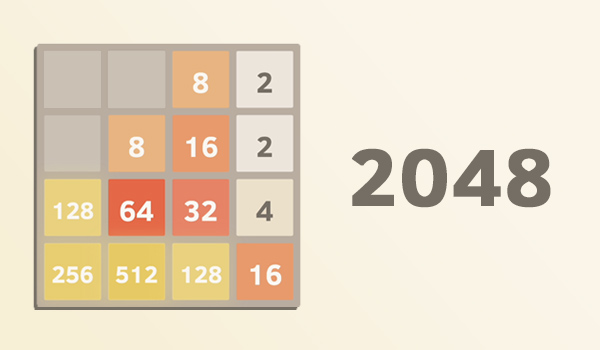
\includegraphics[width=1\linewidth]{2048.jpg}
        \label{fig:2048}
        
        
       
    	\thispagestyle{empty}
	\end{titlepage}

	%\newpage
	
	%\listoffigures
	
	\newpage
	
	$if(abstract)$
	\section*{Résumé}
	$abstract$
	\thispagestyle{empty}
	\clearpage
	$endif$
	
	%Page avec table des matières

	\thispagestyle{empty}
	\tableofcontents
	
	\clearpage
	
	\newpage
	% Redémarrer la numérotation des pages après la table des	 matières
	\pagenumbering{arabic}
	\setcounter{page}{1}
	
    $body$
	
	
\end{document}